% Facultad de Ingenier\'ia, Universidad de Buenos Aires
% 75.59 Técnicas de Programación Concurrente I

\documentclass[a4paper,12pt,titlepage]{article}
\usepackage[paperwidth=180mm,paperheight=285mm,left=1.5cm,top=4cm,right=1.5cm,bottom=2cm,head=2.0cm,includefoot]{geometry}
\usepackage[spanish]{babel}
%\usepackage[latin1]{inputenc}
\usepackage[utf8]{inputenc}
\usepackage{lscape}
\usepackage{graphicx}
\usepackage{fancyhdr}
\usepackage{rotating}
%\graphicspath{{../}}

\usepackage{listingsutf8}

\title{75.59 Técnicas de Programación Concurrente I, Trabajo Práctico 1}
\author{Torres, Miguel \and Montoya, Diego \and Garay, Ignacio}

\lhead{
\includegraphics[scale=0.06]{./logo_fiuba.pdf}}
\chead{ 75.44 - Administraci\'on y control\\ de proyectos inform\'aticos I}
\rhead{}

\lfoot{Torres - Montoya - Garay}
\rfoot{\thepage}
\cfoot{$2^{do}$ Cuatrimestre 2013}

\begin{document}

\thispagestyle{empty}
% T\'itulo del documento.
\begin{center}
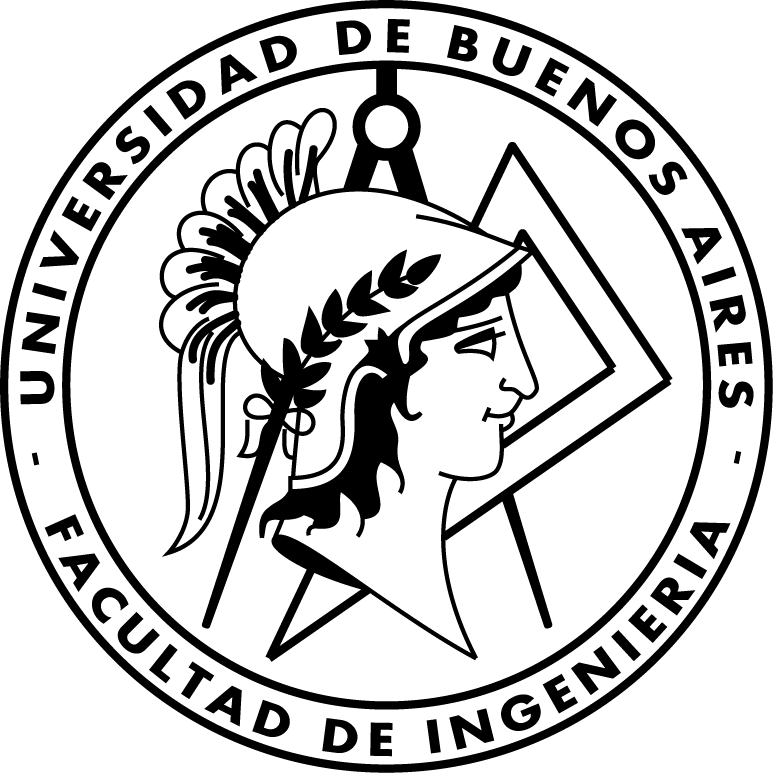
\includegraphics{./logo-fiuba.png}\\
\vspace{1cm}
\textsc{\LARGE Universidad de Buenos Aires}\\[0.3cm]
\textsc{\LARGE Facultad de Ingenier\'ia}\\[1.2cm]
\textsc{\Large 75.59 - Técnicas de Programación Concurrente I}\\[0.3cm]
\end{center}

\begin{flushright}
{\large
Montoya, Diego -- 91939\\
Torres, Miguel -- 91396\\
Garay, Ignacio -- 92265\\
\vspace{2cm}
$2^{do}$ cuatrimestre de 2013}
\end{flushright}

\pagestyle{fancy}
\setcounter{page}{1}
\newpage

\tableofcontents
\newpage

\footnotesize
\section{Análisis}
En el análisis del trabajo se identificaron las siguientes identidades del dominio:\\
\begin{itemize}
\item Aeropuerto
\item Avion
\item Torre
\item Control
\item Pista
\end{itemize}

El aeropuerto se podría entender como la clase que compone la torre y las pistas. El avion interactúa con el
aeropuerto, solicitando un control. Entonces el aeropuerto deriva al avión a la torre de control.
La torre de control posee varios controladores que trabajan independiente de cada uno, conectando los aviones
con las pistas. Las pistas alojan el avión hasta que el mismo ejecuta la tarea que debe, despachándolo.\\

En esta situación se puede apreciar que vamos a necesitar de algun productor de aviones
que vaya generando los aviones correspondientes. El aeropuerto, por caso, haría de consumidor.
El mismo debe derivar los aviones a la torre de control, junto con sus pistas.\\
En esta estructura vemos que se vuelve a repetir el patrón consumidor productor, donde el aeropuerto
viene a ser el productor (asignando el ingreso de aviones), mientras que el consumidor vendría a ser la torre de control.\\


\newpage
\section{Diseño}

Para la resolucion de la concurrencia en la aplicacion se implemenetaron varias herramienstas como Fifo, Lock , Memoria Compartida y Proceso (representa un hilo de ejecucion).

Se crearon los siguientes procesos, uno encargardo de la generacion de aviones, llamado generadorAviones, uno que recibe los aviones creados, llamado consumerAviones, que los coloca en una cola con prioridad, y con otro que se comunica con otro encargado de distribuir los aviones (llamado 
dispatcherAviones).\\

Existe un proceso principal que dispara 2 procesos secundarios, el referido a la generacion de aviones (segun la
cantidad de los mismos en el archivo de configuracion) que luego de crearlos envia estos al proceso que los
coloca dentro de la cola con prioridad.\\

Se decidio realizar un proceso por cada controlador que se necesite, cada avion es entregado por dispatcherAviones a un controlador segun un algoritmo de seleccion, donde luego cada controlador se encarga de elegir alguna Pista que adecuada para completar la accion del avion.\\

Se implemento un sistema de log para hacer un seguimientos de los pasos que vayan haciendo los distintos procesos durante la ejecucion de la aplicacion donde existen distintos niveles de registros para representar distintas situaciones, estos son:
\begin{itemize}
\item Info: informacion corriente de los pasos de la ejecucion.
\item Debug: informacion de debug.
\item Fatal: indica una excepcion lanzada.
\item Warning: informacion de advertencia sobre algun comportamiento anormal.
\item Error: indica un error critico en la aplicacion
\end{itemize}
El archivo de salida de Log esta resguardado por un Lock para su correcta escritura por los distintos procesos que vuelcan su informacion.



\newpage
\section{Diagramas}



\begin{figure}
  \centering
    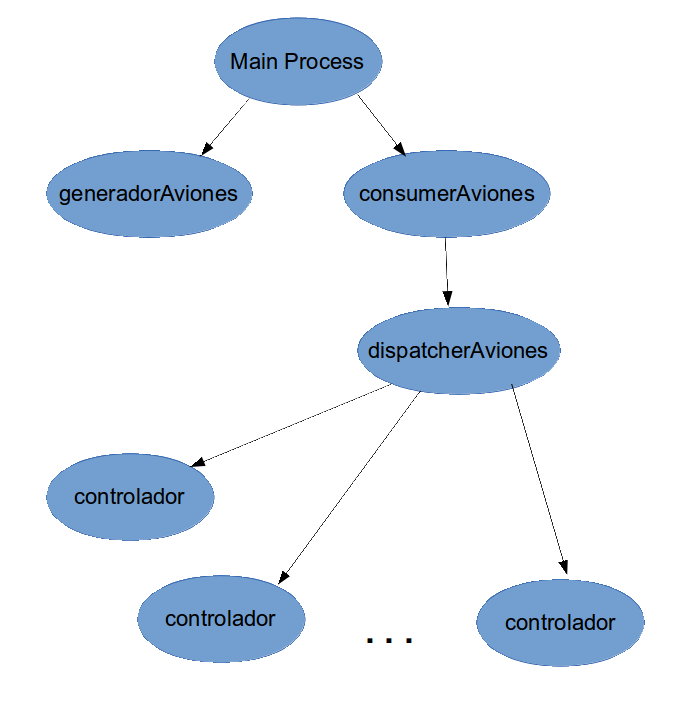
\includegraphics[width=0.6\textwidth] {dia_procesos_2}
  \caption{Diagrama de Procesos.}
  \label{fig:dia_procesos}
\end{figure}


En la Figura~\ref{fig:dia_procesos} se ilustra como es el camino de creacion de los distintos procesos.
Descripcion de los procesos:

\begin{itemize}
\item Main Process: Proceso principal que dispara otros procesos.
\item Generador de Aviones: Genera aviones y los envia a travez de un fifo al consumer.
\item Consumer de Aviones: Recibe aviones del generador y los coloca en la cola de prioridad.
\item Dispatcher de Aviones: Encargado de retirar los aviones de la cola de prioridad y asignar este a un controlador.
\item Controlador: Encargado de llevar a cabo la tarea que debe cumplir un avion, obteniendo una pista para este.
\end{itemize}
\\
% --Diagrama de Comuniacion de procesos--

En la Figura~\ref{fig:dia_comunicacion_procesos} se muestra como es la comunicacion entre los distintos procesos y el medio por el cual se lleva a cabo.

\begin{figure}
  \centering
    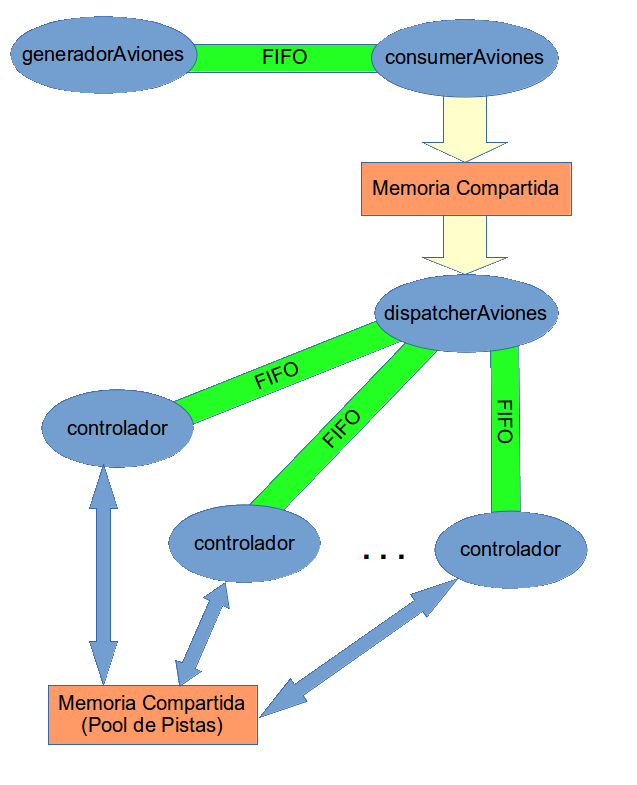
\includegraphics[width=0.6\textwidth] {comunicacion_procesos}
  \caption{Diagrama de Comunicacion entre procesos.}
  \label{fig:dia_comunicacion_procesos}
\end{figure}

% --Diagramas de estados de procesos--


Diagramas de Estados de Procesos

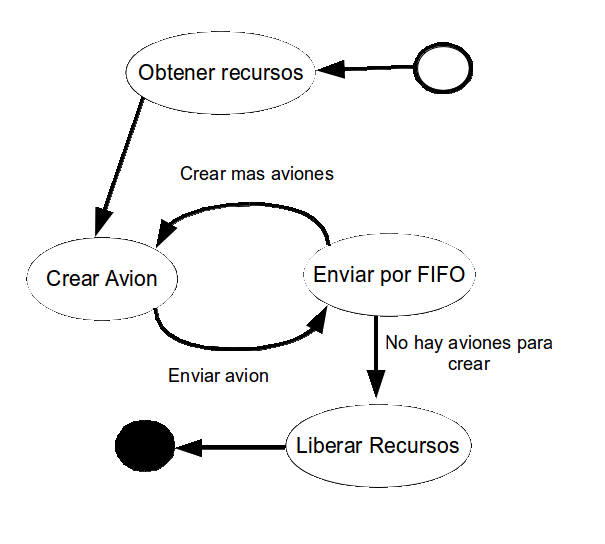
\includegraphics{./dia_est-generadorAviones}\\

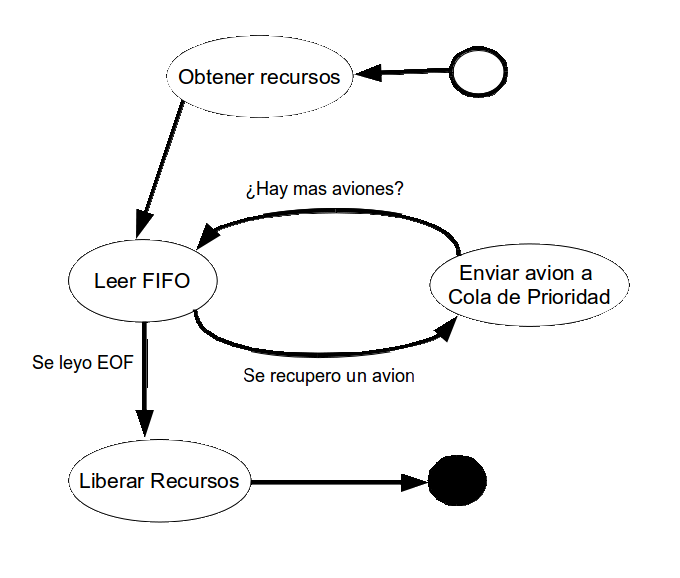
\includegraphics{./dia_est-consumerAviones}\\

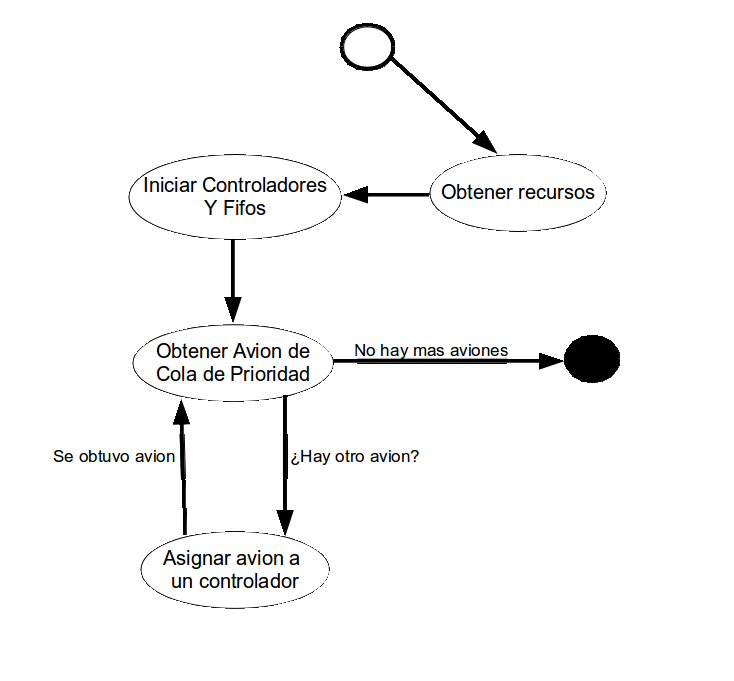
\includegraphics{./dia_est-dispatcherAviones}\\

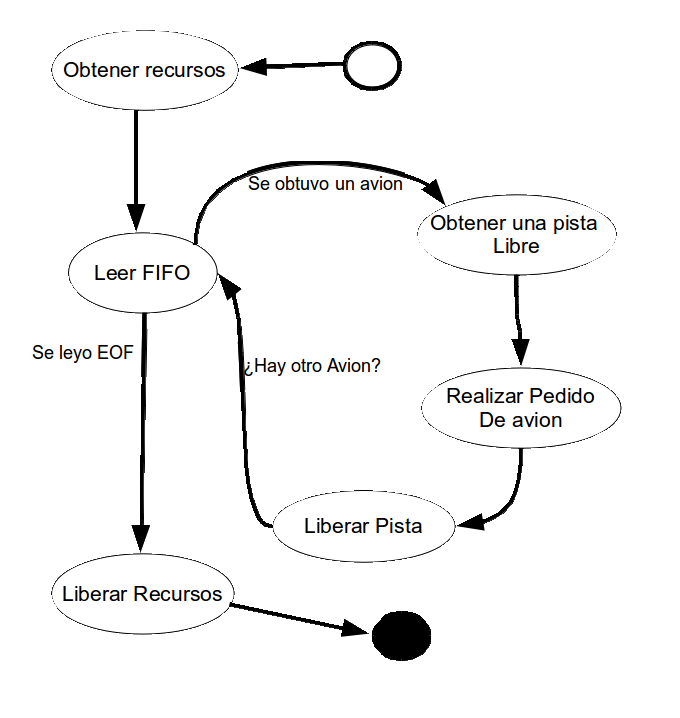
\includegraphics{./dia_est-Controlador}\\

\newpage
\section{Integración}


Los procesos que ''generan'' y ''consumen'' aviones interactuan entre si mediante el usos de Fifos. La comunicacion entre el generadorAviones y el dispatcherAviones se hace mediante el uso de una Memoria Compartida donde en esta se localiza la cola con prioridad de aviones. 

Los aviones que se colocan en la cola de prioridad son representaciones hechas de un avion mediandte por un objeto sencillo que mantiene principalmente su estado(si se encuentra volando o en tierra).

El dispatcher obtiene un avion de la cola, ubicada en la memoria compartida y selecciona un proceso controlador al cual asignarle ese avion mediante un algoritmo particular de seleccion.
Luego de que el controlador obtiene el avion asignado, intenta conseguir una pista vacia para resolver la situacion del mismo, solicitando esta a un gestor de pistas que almacena las pistas libres en una memoria compartia, luego que se consigue realizar la accion del avion se libera la pista(informando al gestor) y se pone a la espera de otra asignacion de algun otro avion. Si no hubiera pista vacias cuando el proceso la solicita se bloquea esperando hasta que alguna se libere.\\


Dentro de un archivo de configuracion se establece las cantidades correspondientes a cada entidad del modelo(aviones, controladores y pistas). El archivo se crea mediante un script desarrolado en python, donde se pide el ingreso de las cantidades de objetos a simular.


\end{document}


